% !TEX TS-program = pdflatexmk

\documentclass{beamer}
\usepackage{times}
\usepackage{hyperref}
\usepackage{enumitem}

\mode<presentation>
{
  \usetheme{UAB}
  \setbeamercovered{transparent}
  \setbeamertemplate{headline}{}
  \setbeamertemplate{blocks}[rounded]
  \setbeamertemplate{navigation symbols}{}
}

\DeclareMathOperator*{\argmin}{argmin}
\DeclareMathOperator*{\argmax}{argmax}

\author{Steven Bethard}
\subject{CS 499: Senior Capstone}


\title{Inequality}
\date{}

\begin{document}

\begin{frame}
\titlepage
\end{frame}

\begin{frame}{Quiz}
Campbell (2000) suggests that:
\begin{enumerate}[(A)]
\item<1> Males prefer challenge, debate and collaboration % No; challenge, debate and individual activities
\item<1> Commands like \texttt{grep}, \text{sed} and \text{awk} are gender biased % No; "killing a job", "fatal errors", "crashing"
\item<1> Men prefer ``rapport talk'' while women prefer ``report talk'' % No; the opposite
\item<1> Women were said to ``dominate'' a forum at 50\% of contributions % No; 30%
\item<1-2> Computer labs should schedule a ``women-only'' time
\end{enumerate}
\bigskip
Goodman (2013) reported that:
\begin{enumerate}[(A)]
\item<1> 91\% of Americans have broadband at home % 71\%
\item<1> 66\% of 18-29 year-olds have a laptop; 57\% have a smartphone % reversed: 57% and 66%
\item<1-2> 98\% of the U.S. population has access to 3 Mbps downstream
%100 million people in the U.S. lived in areas where they had access to broadband, but did not subscribe
\item<1> $>$95\% of Fortune 500 companies require online job applications % 80%
\end{enumerate}
\end{frame}

\begin{frame}{Discussion of Campbell (2000)}
What points from Campbell (2000) are now out of date?\\[5em]
% games aimed at girls/women?
What points from Campbell (2000) are still relevant?
% teaching collaborative for women vs. teaching collaborative because it's required in jobs
\end{frame}

\begin{frame}{Learning Styles: Concepts and Evidence (2009)}
% http://dx.doi.org/10.1111/j.1539-6053.2009.01038.x
What is the theory of learning styles?
\pause
\begin{itemize}
\item Different people learn better from different teaching styles
\item E.g. visual vs. verbal
\end{itemize}
\pause
\bigskip
What is wrong with the following experiments?
\begin{itemize}
% students from each group not assigned different teaching styles
\item Survey students, asking what learning style they prefer.
\pause
% students not divided into groups by learning style
\item Randomly assign students to different teaching styles, measure test performance for each style.
\end{itemize}
\pause
\bigskip
Results of literature review:
\begin{itemize}
\item Different people prefer different styles
\item No evidence they learn better from that style
\end{itemize}
\end{frame}

\begin{frame}{Women in Computing - Take 2 (2009)}
%http://cacm.acm.org/magazines/2009/2/19326-women-in-computing-take-2/fulltext
Stats on women in CS:
\begin{itemize}
\item[+] undergrad degrees: 7,000 in 1995 $\rightarrow$ 11,000 in 2005
\item[+] doctoral degrees: 16.5\% in 1997 $\rightarrow$ 19.8\% in 2005
\item[+] full professors: 5\% in 1995 $\rightarrow$ 10.9\% in 2007
\pause
\item[--] undergrad degrees: 37\% in 1985 $\rightarrow$ 22\% in 2005
\item[--] intention to major in CS: 2.8\% in 1985, 1.3\% in 1995, 0.4\% in 2006
\item[--] employed in math and CS: 33\% in 1984 $\rightarrow$ 27\% in 2004
\end{itemize}
\end{frame}

\begin{frame}{Women in Computing - Take 2 (2009)}
%http://cacm.acm.org/magazines/2009/2/19326-women-in-computing-take-2/fulltext
A sample of initiatives for women in technology:
\begin{itemize}
\item \href{http://girlsgotech.org}{Girls Scouts' Girls Go Tech}
% http://www.girlscoutsnorcal.org/pages/events/ggt.html
% http://vimeo.com/73735417
\item \href{http://engineering.union.edu/edge/}{Educating Girls for Engineering (EDGE) Workshop at Union College}
\item \href{http://women.acm.org/}{ACM Committee on Women in Computing}
\item \href{http://www.google.com/anitaborg/}{Google Anita Borg Memorial Scholarship}
\item \href{http://dx.doi.org/10.1145/1734263.1734281}{Harvey Mudd College course restructuring}
% Switched from Java to Python; split intro course into "standard" and "enrichment" tracks
% Offered trips for first year students to Grace Hopper Celebration of Women in Computing
% Undergraduate research experiences for sophomores
% Also: http://www.npr.org/blogs/alltechconsidered/2013/05/01/178810710/How-One-College-Is-Closing-The-Tech-Gender-Gap
\item Teaching pair programming (\href{http://cacm.acm.org/magazines/2006/8/5850/fulltext}{11.1\% $\rightarrow$ 46.3\% declare CS major})
\item \href{http://cra-w.org/dreu}{CRA-W's Distributed Research Experiences for Undergraduates}
\item National Science Foundation criteria 2: broadening participation of underrepresented groups in STEM
\end{itemize}
\end{frame}

\begin{frame}{Discussion of Goodman (2013)}
\begin{itemize}
\item Who have you met that doesn't have internet access?
\bigskip
\item \href{http://www.openwifispots.com/FinderDirectoryCity.aspx?City=Birmingham&State=AL}{Where can you go for free internet access?}
\end{itemize}
\end{frame}

\begin{frame}{Decline of Print Media}
% http://www.theguardian.com/media-network/media-network-blog/2013/jan/02/end-newsweek-digital-evolution-rosenblum
\begin{columns}
\begin{column}{0.5\textwidth}
History:
\begin{itemize}
\item 1933 - Launched by former editor of Time
\item 1961 - Bought by Washington Post Company
\item 2009 - Refocused on opinion/commentary; 50\% decline in subscriptions
\item 2010 - Merged with online publication The Daily Beast
\item 2013 - End of US print versions
\end{itemize}
\bigskip
\uncover<2->{Does this affect the Digital Divide?}
\end{column}
\begin{column}{0.45\textwidth}
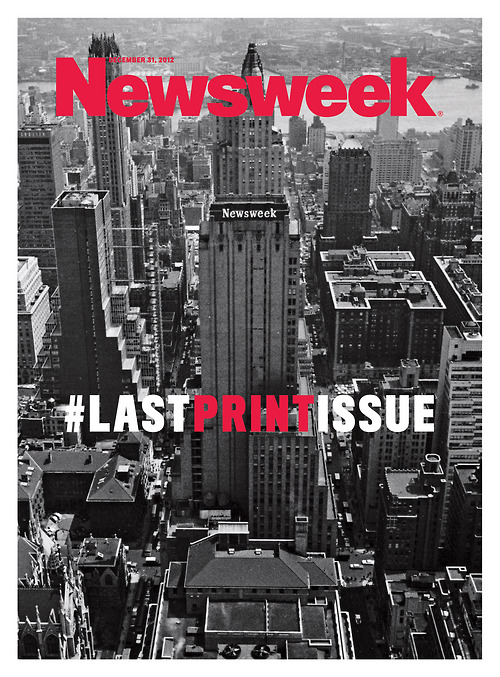
\includegraphics[width=\textwidth]{Newsweek_final_issue.jpg}
\end{column}
\end{columns}
\end{frame}

\begin{frame}{Digital Textbooks}
\href{http://www.youtube.com/watch?v=UB2RXPqFgdI}{A High School Without Textbooks}\\
\bigskip
How would the different factors interact with the Digital Divide?
\begin{itemize}
\item Cost to schools?
\item Cost to students?
\item Alternate learning strategies?
\item One-on-one interactions?
\item Weight of backpacks?
\item Social media distractions?
\end{itemize}
\end{frame}

\end{document}
